 
\section{Problem 1}
\label{part1}
\begin{verbatim}
1.  Choose a blog or a newsfeed (or something similar with an Atom
or RSS feed).  Every student should do a unique feed, so please
``claim'' the feed on the class email list (first come, first served).
It should be on a topic or topics of which you are qualified to
provide classification training data.  Find something with at least
100 entries (or items if RSS).

Create between four and eight different categories for the entries
in the feed:

examples: 

work, class, family, news, deals

liberal, conservative, moderate, libertarian

sports, local, financial, national, international, entertainment

metal, electronic, ambient, folk, hip-hop, pop

Download and process the pages of the feed as per the week 12 
class slides.

Be sure to upload the raw data (Atom or RSS) to your github account.
\end{verbatim}

\subsection{Solution}

\begin{enumerate}
\item I started doing this problem by first searchin for a blog which gives me minimum 100 feeds.
\item It became very tough for me to find a blog like that, Finally I have found this page ``http://www.thehindu.com/news/national/?service=rss'' with minimum of 100 rss feeds.
\item There were more than 100 rss feeds, but I picked only 100 from them and saved it in an xml file. Sample xml file can be seen in fig\ref{Sample1}.
\item Once I got these feeds I have read all of those titles and description of each feed and then I categorized them into the following categories.
\item Accident- Anything that is attacked,killed,injured,any loss happened,any illness or any one arrested. All these situations are categorized into accident category.
\item law- Any anouncement from supreme or high courts,any legal statements are categorized into law category.
\item politics-  Any minister,government and its anouncements and activities are categorized into politics category.
\item elections- Any votings,campaigns,candidates,polls are categorized into elections category.
\item entertainment- Any anouncement regarding films,any happy moments,movies,songs,celebrations are categorized into entertainment category.
\item others- All those which do not come in above categories are categorized into others category.
\item transportation- Any information regarding buses,trains,travel details,traffic are categorized into transportation category.
\end{enumerate}
\newpage

\subsection{Outputs}

\subsubsection{Sample Blog XML file}
\begin{figure}[ht]    
    \begin{center}
        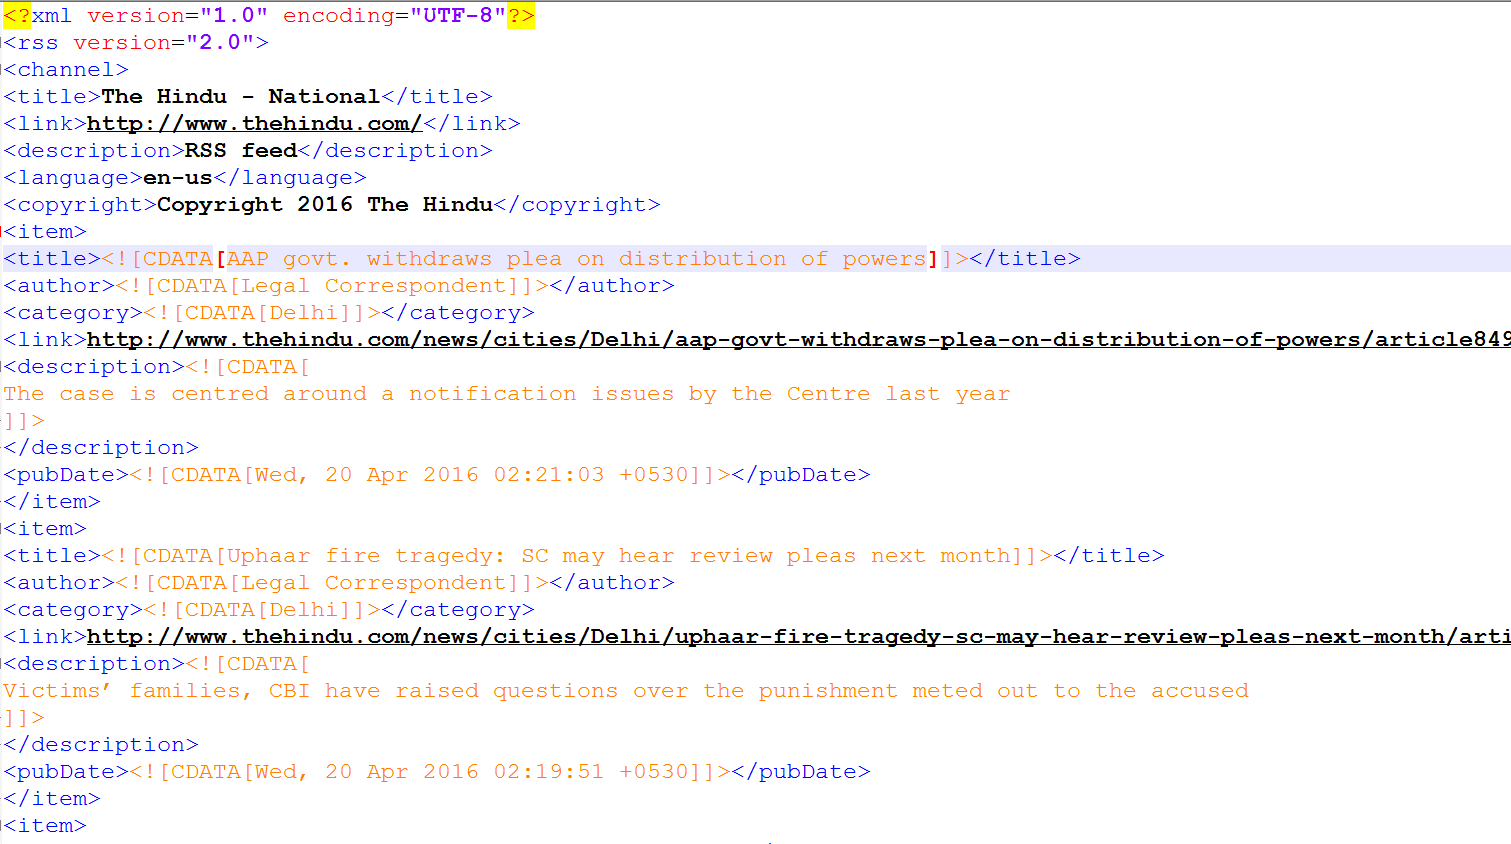
\includegraphics[scale=0.4]{sample_xml.png}
        \caption{Sample list of Blog Feeds}
        \label{Sample1}
    \end{center}
\end{figure}
\newpage
